% Created 2019-10-07 Mon 02:30
% Intended LaTeX compiler: pdflatex
\documentclass[11pt]{book}
\usepackage[utf8]{inputenc}
\usepackage[T1]{fontenc}
\usepackage{graphicx}
\usepackage{grffile}
\usepackage{longtable}
\usepackage{wrapfig}
\usepackage{rotating}
\usepackage[normalem]{ulem}
\usepackage{amsmath}
\usepackage{textcomp}
\usepackage{amssymb}
\usepackage{capt-of}
\usepackage{hyperref}
\usepackage{helvet}
\usepackage{gensymb}
\usepackage{xcolor}
\usepackage{appendix}
\usepackage{tikz}
\usepackage{microtype}
\renewcommand{\familydefault}{\sfdefault}
\linespread{1.5}
\usepackage{tabularx}
\usepackage{tabu}
\usepackage[margin=1.4in]{geometry}
\usepackage[sort&compress,numbers]{natbib}
\usepackage[font=small,labelfont=bf]{caption}
\setcounter{secnumdepth}{2}
\author{\textbf{Student:} Jamin Wu \\ \textbf{Student ID:} 27025861 \\ \\ \textbf{Supervisor:} Dr Yan Tat Wong \\ \textbf{Co-Supervisor:} Dr Nicholas Price \\ \\ Department of Physiology \\ Department of Electrical \& Computer Systems Engineering \\ \textbf{School of Biomedical Sciences, Monash University} \\ \\ Minor thesis submitted in partial fulfillment of the requirements for the \\ degree Bachelor of Medical Science (Honours) at Monash University. \\ \\ Word Count: <> words}
\date{}
\title{\textbf{Using Generative Adversarial Networks to Derive Phosphene Patterns in Simulated Prosthetic Vision}}
\hypersetup{
 pdfauthor={\textbf{Student:} Jamin Wu \\ \textbf{Student ID:} 27025861 \\ \\ \textbf{Supervisor:} Dr Yan Tat Wong \\ \textbf{Co-Supervisor:} Dr Nicholas Price \\ \\ Department of Physiology \\ Department of Electrical \& Computer Systems Engineering \\ \textbf{School of Biomedical Sciences, Monash University} \\ \\ Minor thesis submitted in partial fulfillment of the requirements for the \\ degree Bachelor of Medical Science (Honours) at Monash University. \\ \\ Word Count: <> words},
 pdftitle={\textbf{Using Generative Adversarial Networks to Derive Phosphene Patterns in Simulated Prosthetic Vision}},
 pdfkeywords={},
 pdfsubject={},
 pdfcreator={Emacs 26.1 (Org mode 9.2.4)}, 
 pdflang={English}}
\begin{document}

\maketitle
\clearpage

\section*{Abstract}

\clearpage

\section*{Acknowledgements}

\clearpage

\section*{Declaration}

\clearpage

\setcounter{tocdepth}{3}
\tableofcontents

\chapter*{List of Abbreviations}

\begin{description}
\item[{CGAN}] conditional generative adversarial network
\item[{CVP}] cortical visual prosthesis
\item[{GAN}] generative adversarial network
\item[{ReLU}] rectified linear unit
\end{description}

\listoftables
\listoffigures

\part{Background}
\label{sec:org8ef7dd2}
\chapter{Introduction}
\label{sec:org00ab7df}

Blindness is a significant disability and can be caused by damage at any point along the visual pathway from the eye to the brain.
A \textbf{cortical visual prosthesis} (CVP) is a vision-restoring device inserted directly into the brain, replacing all parts of the visual pathway except the brain itself.
Because a CVP only requires a functioning brain, CVPs are a flexible (and potentially the only) option for many causes of non-cortical blindness.

However, a significant detractor from CVPs is that they are currently only expected to provide very low-quality vision.
As CVPs are still in early development with clinical trials only beginning to emerge, we still do not know exactly what people will be able to see.
What \emph{is} known is that people tend to see small spots of light called \textbf{phosphenes} - like "stars in a night sky" - when small regions of the brain are stimulated.
Unfortunately, we cannot yet reliably control the locations of phosphenes, nor their qualities beyond simply being "on" or "off".

To address the perceptual limitations of CVPs, a large body of research has been devoted to investigating how image processing techniques can make phosphenes meaningful.
These include using phosphenes to selectively display salient objects, display only prominent edges, or even replacing faces with low-resolution icons.
However, most of these studies are premised on static, optimistic simulations of prosthetic vision.
Many do not address how to apply traditional image processing strategies when we cannot control how phosphenes are laid out or what qualities they possess.
As a result, it is not clear what methods can be used to generalise image processing strategies to different people, who experience phosphenes differently.

Outside of prosthetic vision, there have been advances in using computers to generate novel imagery under specified conditions.
\textbf{Generative adversarial networks} (GANs) are a machine learning technique to generate new data samples (most often, images) when given many examples of data known prior.
GANs are not an image processing algorithm \emph{per se}, but a method of training a neural network to take a seed input and return a generated data sample.
GANs work by optimising the features of generated data samples to be as indistinguishable from real data samples as possible.
They have been used with varying degrees of success in a number of scene generation, style transfer and image processing tasks.

Because GANs are used to make generated images look more realistic, it is possible they could be used in a prosthetic vision setting to make phosphene patterns look more like what they are supposed to represent.
Importantly, GANs are a \emph{training} technique which can be applied to different types of phosphene simulations to produce specifically-tailored results.
This means GANs may be able to address the difficulties in finding generalised image processing strategies suitable for different people's experiences of prosthetic vision.

To our knowledge, there are no prior studies which attempt to apply GANs to the problems faced by prosthetic vision.
The following chapters review the literature surrounding CVPs, the visual percepts they produce, and previous approaches to addressing these limitations.

\chapter{Project Motive}
\label{sec:orgca01afd}

\section*{Research Questions}
\label{sec:org4568c3f}

As there are no prior studies applying GANs to simulated prosthetic vision, this project aimed to address the following research questions::

\begin{enumerate}
\item Can GANs be used to train a neural network to produce phosphene patterns representing digits, given different simulated properties of prosthetic vision and, if so, how could this be implemented?
\item Do people find it easier to recognise digits from phosphene patterns derived from training via GANs, compared to a basic comparison (directly masking digits with a phosphene grid)?
\end{enumerate}

\section*{Aims and Hypothesis}
\label{sec:orgde30108}

To address the two research questions, this project aimed to:

\begin{enumerate}
\item Develop a preliminary software implementation of a GAN training architecture for generating phosphene patterns, which could be applied to different phosphene simulations with minimal modification.
\item Experimentally test whether people find it easier to recognise digits from phosphene patterns derived from our prototype training implementation, compared to a basic mask-based comparison.
\end{enumerate}

Aim 2 relies on the implementation produced in Aim 1 and can be hypothesis-tested against the folowing hypothesis:

\begin{enumerate}
\item Sighted participants, under simulated conditions, have a higher overall digit recognition accuracy when viewing phosphene patterns derived from our prototype GAN training architecture, compared to when viewing phosphene patterns produced by basic image processing using masking.
\end{enumerate}

\section*{Rationale}
\label{sec:org0e1c73b}

While GANs have been applied to image-based tasks in other domains, it is not yet clear how they should be applied to prosthetic vision.
An important difference between GANs in other domains versus prosthetic vision is that typically GANs directly manipulate every pixel in images they generate.
This gives GANs complete control over what its generated images look like and it can optimise the output of each individual pixel.

However, this is not desirable in simulated prosthetic vision where we want to simulate visual experiences which we \emph{cannot} fully control.
GANs must instead be used to generate \emph{instructions} to simulated electrodes, which produce a simulated visual render independent of the GAN based on specified simulation properties.
A useful GAN implementation for simulated prosthetic vision should therefore \emph{not} be based on direct pixel manipulation (as is typically the case).

Aim 1 therefore aims to explore and develop a useful GAN implementation based on separating out a simulated rendering step so that it can be applied to simulated prosthetic vision.
This is the primary contribution of this project.

GANs are designed to minimise the computer's ability to discriminate between generated images and real image samples.
However, computers both find it easy to discriminate features which humans find difficult (e.g. different shades of grey) and find it difficult to discriminate features which humans find easy (e.g. abstract scenes).
As a result, while the generated output may be optimised for a computer, its results may not translate to a human.
Aim 2 is therefore formulated as a preliminary validation measure to test whether the computer's output was human-benefitting.

Aim 2 is \emph{not} intended to provide conclusive or compelling evidence on the usefulness of GANs in general for simulated prosthetic vision.
It is purely intended as a short-term checkpoint on the performance output of the implementation in Aim 1.
It is not expected that this project will produce a necessarily useful software implementation in Aim 1 given its novelty.
The preliminary validation results may instead be used to guide how to better refine the software implementation for future use.

\part{Methods}
\label{sec:org6b13db8}
\chapter{Methodology Overview}
\label{sec:org08f06b5}

This project involved two stages:

\begin{enumerate}
\item Development of a software implementation of a GAN training architecture to derive phosphene patterns of digits, for different types of phosphene simulation properties.
\item Implementation and conduct of a psychophysics experiment to test GAN-trained phosphene patterns (using the implementation developed in the first stage) against basic mask-based controls for a digit recognition task.
\end{enumerate}

\chapter{Development of GAN Training Architecture}
\label{sec:org82d09ce}
\section*{Development Context}
\label{sec:org60bfeb3}

The code required for this project was written by the author using the Python programming language.
Where appropriate, some snippets of code have been included below; the remainder of the codebase is too large for inclusion in this manuscript and is therefore hosted and available for perusal at the following GitHub repository (TODO).
All code was developed on a Windows 10 personal computer.
Code was executed both on the development computer (Windows 10) and remotely on the M3 MASSIVE high-performance-computing platform.

\begin{itemize}
\item[{$\square$}] TODO: Host code on GitHub repository (+/- include several files in appendices)
\end{itemize}

\section*{Overview}
\label{sec:org0aa64c8}

A high-level overview of the implemented GAN training architecture is provided in Figure \ref{fig:org3e45fac}.

\begin{figure}[htbp]
\centering
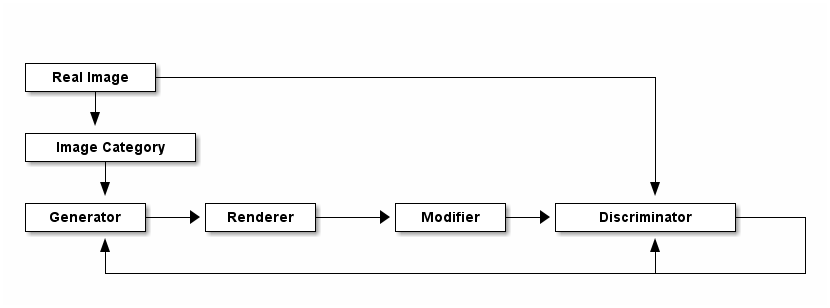
\includegraphics[width=.9\linewidth]{images/methods_training_architecture.png}
\caption{\label{fig:org3e45fac}
Overview of GAN training architecture implementation.}
\end{figure}

This architecture closely follows classical GAN architectures (explicitly, a conditional GAN architecture), with the addition of the \emph{Renderer} and \emph{Modifier} steps.
The flow of data through the training proceeds as:
\begin{enumerate}
\item A \emph{Renderer} is first chosen for this training run.
The \emph{Renderer} corresponds to a parametric phosphene simulator, which can be altered for different training runs.
\item A real image sample of a digit is taken from a pool of real digits.
\item The image category (in this case, the identity of the digit e.g. a "3") of the image sample is taken from its label.
\item The image category is fed into the \emph{Generator}, which produces a set of instructions - an image \textbf{encoding} - for the \emph{Renderer}.
\item The \emph{Renderer} takes the encoding and simulates it as phosphenes, producing a simulated prosthetic vision image.
\item The \emph{Modifier} takes the simulated prosthetic vision image and modifies it to more closely align it with the domain of the real images.
This is discussed further in the sections below.
\item The \emph{Discriminator} takes both real images, and modified simulated prosthetic images and produces predictions of the digit identity and whether it was real or fake.
The difference of its predictions from the true identities of each image is used to adjust the \emph{Generator} and \emph{Discriminator} to better perform their tasks.
\end{enumerate}

As with classical GAN architectures, the \emph{Generator} and \emph{Discriminator} participate in a zero-sum game where each network has opposing goals; the \emph{Generator} aiming to fool the \emph{Discriminator} into thinking its \emph{Rendered} encodings are real, and the \emph{Discriminator} aiming to identity the \emph{Generator}'s fakes amongst the real samples.

This process is repeated many times to slowly optimise the \emph{Generator} to produce useful encodings that can be fed to the renderer to produce digit-like phosphene patterns.
Each step of this process is discussed in further detail in the sections below.

\section*{Real Images}
\label{sec:org79c4924}

The \emph{Generator} begins training as a naive neural network with no conception of what digits are or what they look like.
In order for the \emph{Discriminator} to train the \emph{Generator} to produce digit-like encodings, the \emph{Discriminator} must be provided samples of what real digits actually look like.

This project used handwritten digit samples from the public MNIST digit dataset. \cite{Lecun1998}
The MNIST digit dataset consists of 60,000 grayscale images stored as 2D pixel arrays with dimensions 27x27 pixels.

The MNIST digits are advantageous because:
\begin{enumerate}
\item It is a publicly-available, comprehensive, labelled, clean, and well-validated dataset (indeed, often the \emph{de facto} dataset for benchmarking machine-learning tasks).
\item Handwritten digits ensure there is sufficient variation within the dataset so that the \emph{Generator} and \emph{Discriminator} are incentivised to learn general features of digits (as opposed to rote-memorising whole digits, as might occur with using digits in a standard font).
\end{enumerate}

Samples of the raw MNIST digit dataset are provided in Figure \ref{fig:org593149f}.

\begin{figure}[htbp]
\centering
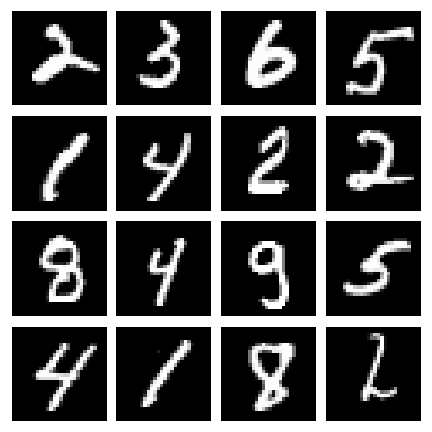
\includegraphics[width=.9\linewidth]{./images/mnist_samples.png}
\caption{\label{fig:org593149f}
16 randomly-selected digits from the MNIST handwritten digit dataset.}
\end{figure}

In order for the \emph{Discriminator} to produce useful optimisations, there must be no obvious systematic difference between renders produced by the \emph{Renderer} and the real images.
If such systematic differences were present, the \emph{Discriminator} would have no difficulty discriminating real and generated images and the \emph{Generator}'s output would therefore shift aimlessly as it tries to converge to an impossible goal.

A series of adjustments were therefore performed on the real images to mitigate systematic differences with images achievable by the \emph{Renderer}.
In order to more faithfully simulate a single unilateral cortical prosthetic vision device, we restricted renders to a single half of the visual fields (the right visual field).
We therefore conducted the same adjustment to the MNIST digits by scaling each images' width by half and aligning the result with the right array edge.
Each image's pixel value was also rescaled between -1 and 1 (from 0 to 255) to improve stability of the neural network output and the entire image upscaled to a resolution of 48x48 pixels to equal the pixel resolution of simulated renders.
These adjustments to the real image dataset are illustrated in Figure (TODO).

\begin{itemize}
\item[{$\square$}] TODO: Figure showing adjustments
\end{itemize}

\section*{Image Category}
\label{sec:org617e7cf}

The MNIST digit dataset includes a digit label for each handwritten data image in the range 0-9 inclusive.
These image categories are simply encoded as an integer corresponding to their digit label.
As integers (i.e. a numerical datatype), these image categories are suitable for direct input into the \emph{Generator}.

\section*{\emph{Generator}}
\label{sec:org9597c77}

The \emph{Generator} is a neural network which:

\begin{itemize}
\item Takes a single digit in the range 0-9, and
\item Returns instructions to each simulated electrode, as a vector of floating-point numerical values equal in length to the number of electrodes in the simulated prosthesis.
\end{itemize}

There is a notable difference in the \emph{Generator} network described above compared to traditional \emph{Generators} in GANs: the lack of a random seed input.
This was an intentional choice.
The use of a random input seed into \emph{Generator} networks in GAN architectures allows it to output multi-modal images - i.e. images which are similarly realistic, but possess slight image variations.
This is often desirable, where we want GANs to produce many different novel images instead of just one.

However, for use in simulated prosthetic vision, multi-modal output is a low priority.
Firstly, the ability to incorporate multi-modality into a \emph{Generator} which does \emph{not} have direct access to its final render is not clear.
Secondly, it may actually be desirable to limit the output to one "good" phosphene pattern per digit; in practice, subjects are likely to find it easier to learn one phosphene pattern per digit only rather than having to deal with many "similar" patterns with extra variable features.

Because this is the first attempt at developing a GAN for our purpose, it is unknown what neural network architecture is best suited for this task.
Our task consists of a simple mapping between 10 image categories (digit identities) to deterministic vectors as we purposefully removed the usual random seed input.
We therefore used a neural network with a minimal number of hidden layers to reduce training times, depicted in Figure (TODO).

The \emph{Generator} network consisted of:
\begin{enumerate}
\item An \emph{input} layer, containing a single neuron taking a digit from 0-9 as input.
\item An \emph{embedding} layer, which maps the single categorical digit class into a 10-element continuous vector.
\item A \emph{batch normalization} layer, which applies a normalisation for each mini-batch before feeding into the next layer.
\item A \emph{leaky ReLU} layer, which applies a rectifier activation function to dampen negative values.
\item A \emph{dense} layer, which outputs a vector of simulated electrode instructions for a specified number of electrodes.
\item A \emph{sigmoid} layer, which applies a sigmoid activation function to constrain all output values between 0 and 1.
\end{enumerate}

My passing an image category (digit 0-9) into the \emph{Generator} as input, the \emph{Generator} therefore outputs a vector of simulated electrode instructions according to the specified number of electrodes.
The simulated electrode instructions take the form of a vector of floating-point numbers between 0 and 1 inclusive, with the number of elements equalling the number of electrodes.
Each floating-point number indicates the "brightness" at which an electrode should be activated to represent a particular image category (digit).
Notably, there is no information encoded about what electrode actually \emph{does}, nor where it is located; the \emph{Generator} network is effectively blind to these elements of the simulation.

\begin{enumerate}
\item[{$\square$}] TODO: Graphical depiction of the encoder network
\end{enumerate}

\section*{Renderer}
\label{sec:org0633bed}

The \emph{Renderer} is a custom simulation of prosthetic vision, which takes instructions for each "electrode" as input, and outputs the simulated render as a grayscale image.
The \emph{Renderer} is a simulated stand-in for real implantees and their perception of vision through a CVP.

The \emph{Renderer} is essentially a 3D volume of pre-rendered 2D grayscale image slices, each slice corresponding to the visual percept of a single electrode.
These pre-rendered grayscale slices allow each electrode to produce a distinct, unique percept; for example, one electrode in the \emph{Renderer} may produce a small phosphene located near the center of vision, while another may produce a much larger phosphene in the peripheries.
When an instruction for each electrode is supplied, each slice in the 3D volume is weighted according to its value.
The slices are then aggregated together by summing along the long axis, and clipping values between 0 and 1 to produce a final grayscale render.
The final render is then rescaled between -1 and 1 before being supplied to the discriminator.
This process is visualised in Figure (TODO).

\begin{itemize}
\item[{$\square$}] TODO: Graphic visualisation of the renderer
\end{itemize}

Because the \emph{Renderer} base is a 3D volume of pre-rendered slices, different subjects can be simulated by using different pre-rendered volumes without requiring changes to the rendering process.
In addition, the use of pre-rendered slices makes training much more efficient, as creating the render consists merely of bulk matrix operations which are easily vectorisable.

In order to generate test grids for use with training, two different means of generating pre-rendered slices were implemented:
\begin{enumerate}
\item Cartesian-spaced phosphenes, which maps electrodes to positions in a regular Cartesian plane and assigns the same size and strength to each phosphene.
This was chosen as a basic control as this grid essentially approximates a normal (albeit low-resolution) pixel image.
\item Polar-spaced phosphenes, which maps electrodes to positions in a regular Polar grid and assigns to each phosphene a size corresponding to its location, as given by the equation \(log(k \times (x^2 + y^2) + a)\) for parametrically-set values \(k\) and \(a\).
This was chosen to more closely reflect the visual qualities of phosphenes known to appear to subjects from experimental trials of cortical stimulation.
\end{enumerate}

For each of the two implementations above, two optional flags were also added:
\begin{enumerate}
\item A randomising flag, which produces phosphenes at random locations instead of along a regular Cartesian or Polar grid.
\item A half-flag, which constrains phosphenes to appear only in a single half of the visual fields (simulating a single implant, inserted into only one hemisphere of the brain).
\end{enumerate}

These grids are illustrated in Figure (TODO).

\begin{itemize}
\item[{$\square$}] Graphic visualisation of layouts of the grids described in this step!
\end{itemize}

\section*{Modifier}
\label{sec:org674f96a}
\section*{Discriminator}
\label{sec:org8626dd4}
\section*{Training Cycles}
\label{sec:orge7eca6f}

\chapter{Psychophysics Experiment}
\label{sec:org5606157}
\section*{Development}
\label{sec:orgc01aa4c}
\section*{Recruitment}
\label{sec:orgd15dd4b}
\section*{Setting}
\label{sec:org413193f}
\section*{Conduct}
\label{sec:org5c2b0a3}
\section*{Analysis}
\label{sec:org78ce417}

\clearpage

\part{Results}
\label{sec:org6ad2c6f}

The results are divided into:

\begin{enumerate}
\item Training results, showing qualitative phosphene patterns and training statistics of digit encoders produced by training, and
\item Experimental results, derived from participants' performance during the psychophysics experiment described in Section <>.
\end{enumerate}

\section*{Training Results}
\label{sec:org51e4b6a}

The cGAN training architecture described in Section <> was tested on a large variety of phosphene grids varying in phosphene location, sizing, regularity and resolution.
We have selected a representative sample of grids to highlight several general features of the training results.

\begin{itemize}
\item Generalisability of Training
\label{sec:orge0af37b}

We were successful in applying the training process to different types of phosphene grids, which varied primarily in spatial distribution, phosphene size and phosphene resolution.

Figure <> shows the phosphene patterns for the digits 0-9 after 20 epochs of training for a regular cartesian grid, a regular polar grid, and a randomised polar grid, each with 144 phosphenes.

<FIGURE <>>

There were no issues applying the training architecture to grids with arbitrary arrangements and resolutions.

\item Stability of Phosphene Patterns over Epochs
\label{sec:org3685ede}

Phosphene patterns were not stable over epochs; i.e. the phosphene patterns learned by the trained encoder always changed with the next epoch.

Figure <> shows the trained phosphene representation for the digits 0-9 for a random grid with 144 phosphenes over each of 40 epochs.

<FIGURE <>>

For comparison, Figure <> shows the equivalent results of Figure <>, trained for a different random grid of only 64 electrodes.

<FIGURE <>>

From these figures, it is evident that:

\begin{enumerate}
\item The degree of instability reduces (but does not disappear) as the number of epochs increases.
\item The qualitative consequences of instability are greater at low resolution.
Small changes in the moderate resolution patterns usually do not disturb the overall form of the digit from one epoch to the next (though the overall form may eventually drift over multiple epochs).
However, small changes in low resolution patterns greatly influence the digit form produced by phosphenes, resulting in a relatively higher impact of instability.
\end{enumerate}
\end{itemize}

\section*{Experimental Results}
\label{sec:org5e02e33}

All 11 participants were included in the analysis.
All participants provided at least one complete block each of digit recognition data for both the control processor and the trained encoder for their grid.
All data was considered valid and included in the analysis.

\begin{itemize}
\item Overall Accuracy
\label{sec:org98890eb}

\begin{itemize}
\item Pooled
\label{sec:org588aeae}

\item By Participant
\label{sec:org0144534}
\end{itemize}

\item Statistical Effects
\label{sec:orga1c123e}

\begin{itemize}
\item Condition
\label{sec:org5e53f6c}

\item Progress
\label{sec:org5d09f8e}

\item Digit
\label{sec:org90ac40d}
\end{itemize}

\item Response Time
\label{sec:orgae492dd}

\item Initial Accuracy
\label{sec:orge7386e2}
\end{itemize}

\part{Discussion}
\label{sec:org7a22174}
\chapter{Relation to Aims}
\label{sec:org98cb18e}
\chapter{Implications}
\label{sec:orgc1fd62b}
\chapter{Limitations}
\label{sec:org059508e}
\chapter{Future Directions}
\label{sec:org521acb7}
\part{Conclusion}
\label{sec:orgdc9136a}
\begin{appendices}
\part{Appendices}
\label{sec:org6eab54b}
\chapter{Additional Qualitative Results: Examples}
\label{sec:org91c8641}
\chapter{Psychophysics Explanatory Statement}
\label{sec:orga39179b}
\chapter{Psychophysics Consent Form}
\label{sec:orgf041404}
\chapter{Selected Code}
\label{sec:orgfa043aa}
\section*{Plotting}
\label{sec:org8c98f39}
\clearpage
\part{References}
\label{sec:orge2fe194}
\bibliographystyle{vancouver}
\bibliography{refs}
\end{appendices}
\end{document}
